\documentclass[aspectratio=169]{beamer}
\useoutertheme[progressbar=frametitle]{metropolis}
\useinnertheme{metropolis}
\definecolor{nabgray}{rgb}{0.6,0.59,0.61}
\usecolortheme[named=nabgray]{structure}
\usepackage{tikz}
\usepackage[utf8]{inputenc}
\usepackage[spanish]{babel}
\usepackage{fontspec}
\setmonofont{JetBrains Mono}
\setmainfont{Roboto}
\setsansfont{Roboto}

\usepackage{smartdiagram}
\usepackage{qtree}
\usepackage{verbatim}
\usepackage{svg}
\usepackage{graphicx}
\usepackage{color}
\definecolor{lightgray}{rgb}{0.95, 0.95, 0.95}
\definecolor{darkgray}{rgb}{0.4, 0.4, 0.4}
\definecolor{ocherCode}{rgb}{1, 0.5, 0} % #FF7F00 -> rgb(239, 169, 0)
\definecolor{blueCode}{rgb}{0, 0, 0.93} % #0000EE -> rgb(0, 0, 238)
\definecolor{greenCode}{rgb}{0, 0.6, 0} % #009900 -> rgb(0, 153, 0)

\usepackage{upquote}
\usepackage{listings}
\lstset{language=java,
    otherkeywords={var,record},
	% Basic design
	backgroundcolor=\color{lightgray},
	basicstyle={\small\ttfamily},
	frame=l,
	keywordstyle=\footnotesize\color{blue},
	escapeinside={<@}{@>},
	breaklines=true,
	% Line numbers
	xleftmargin={0.75cm},
	numbers=left,
	stepnumber=1,
	firstnumber=1,
	numberfirstline=true
	% Code design
	identifierstyle=\color{black},
	keywordstyle=\color{ocherCode}\bfseries,
	ndkeywordstyle=\color{greenCode}\bfseries,
	stringstyle=\color{ocherCode}\ttfamily,
	commentstyle=\color{darkgray}\ttfamily,
	tabsize=2,
	showtabs=true,
	showspaces=false,
	showstringspaces=false,
	extendedchars=true,
	breaklines=true
}

\lstdefinelanguage{bash}{
    basicstyle=\ttfamily,
    showstringspaces=false,
    commentstyle=\color{red},
    keywordstyle=\color{blue},
    numbers=right,
    xleftmargin={0.25cm}
}

\usebackgroundtemplate
{
	
\includegraphics[width=\paperwidth]{Images/fondo}%
}


\title{Actualizando aplicaciones empresariales en Java desde Java 8 on premise hasta Java 11 en la nube}
\author{Víctor Orozco - @tuxtor}
\institute{Nabenik}
\date{\today}

\begin{document}

{
    \usebackgroundtemplate{
\includegraphics[width=\paperwidth]{Images/portada}}
    \setbeamercolor{frametitle}{fg=red}
    \usebeamercolor[fg]{normal text}
    \frame{\titlepage}
}


\begin{frame}
    \tableofcontents
\end{frame}



{
    \usebackgroundtemplate{
\includegraphics[width=\paperwidth]{Images/separador}}
    \setbeamercolor{normal text}{fg=white}
    \setbeamercolor{frametitle}{fg=red}
    \usebeamercolor[fg]{normal text}
    \section{Historias del mundo real}
}
\begin{frame}[fragile]{Un sistema de geocerca}

    \begin{figure}
        \centering
        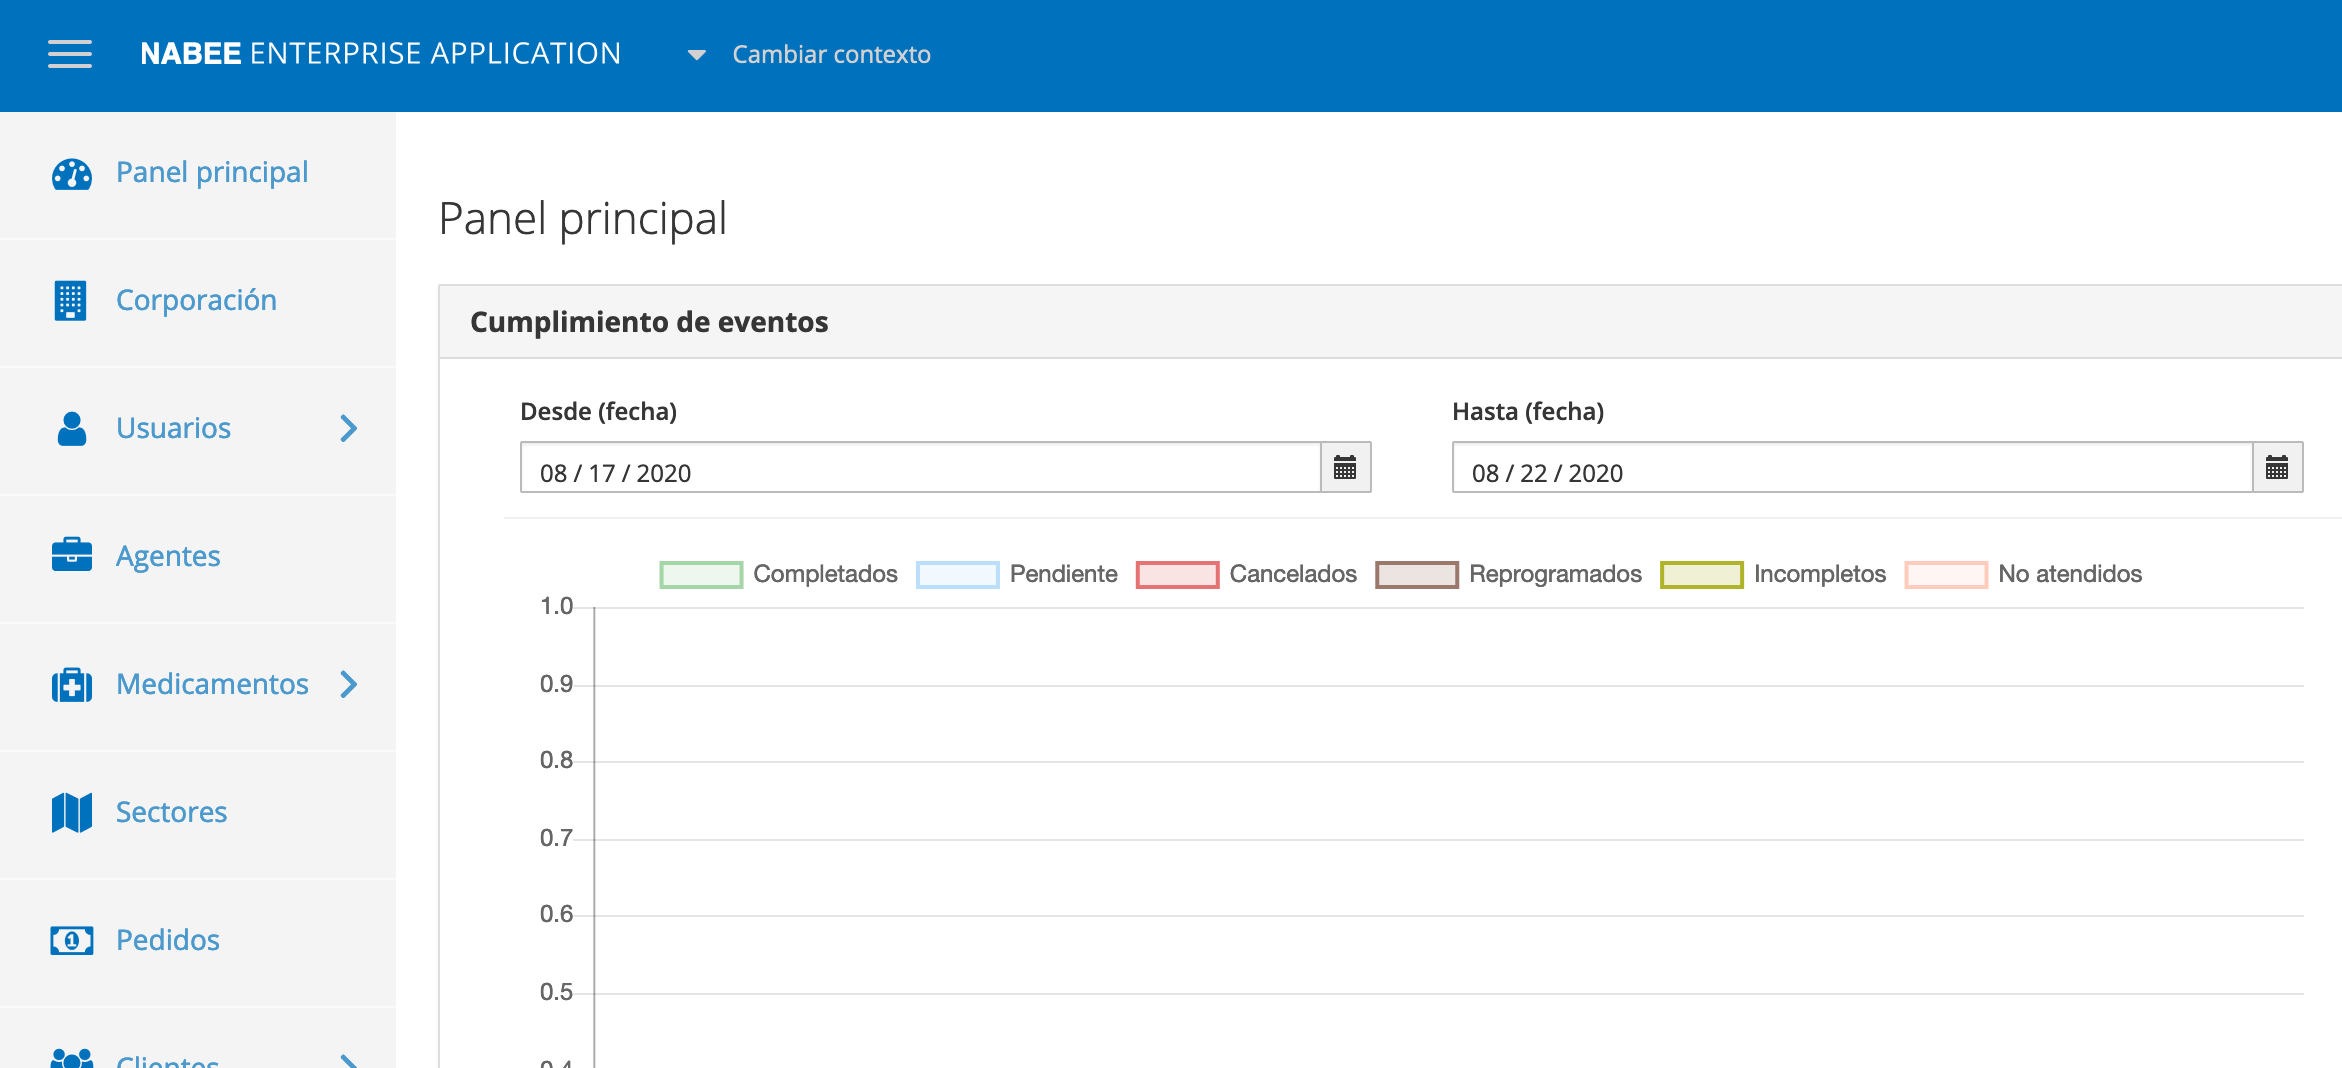
\includegraphics[width=\linewidth]{Images/rep}
    \end{figure}
\end{frame}

\begin{frame}[fragile]{Un sistema de geocerca}
\begin{columns}[T] % contents are top vertically aligned

    \begin{column}[T]{5cm} % alternative top-align that's better for graphics
       \begin{itemize}
       \item 2017
               \item 5 modulos (War/Microservicios)
               \item 348 clases
               \item 17160 lineas de código + dependencias
       \end{itemize}
    \end{column}
    \begin{column}[T]{6cm} % each column can also be its own environment
        \begin{itemize}
           \item Original: Glassfish 4, Java EE 7, Java 8
           \item Actual: Payara 5, Jakarta EE 8, MicroProfile 3.2
           \item Cliente Android y web (Angular)
       \end{itemize}
    \end{column}
\end{columns}
\end{frame}

\begin{frame}[fragile]{Un sistema de geocerca}

    \begin{figure}
        \centering
        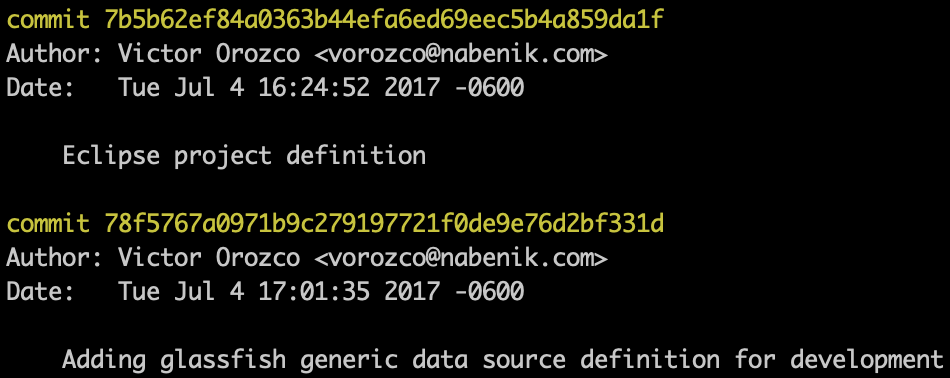
\includegraphics[width=\linewidth]{Images/fcommit}
    \end{figure}
\end{frame}

\begin{frame}[fragile]{Un sistema de geocerca}

    \begin{figure}
        \centering
        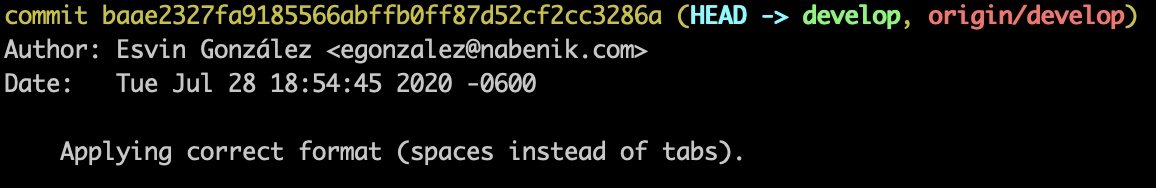
\includegraphics[width=\linewidth]{Images/lcommit}
    \end{figure}
\end{frame}


\begin{frame}[fragile]{Un - sistemita - contable y empresarial}

    \begin{figure}
        \centering
        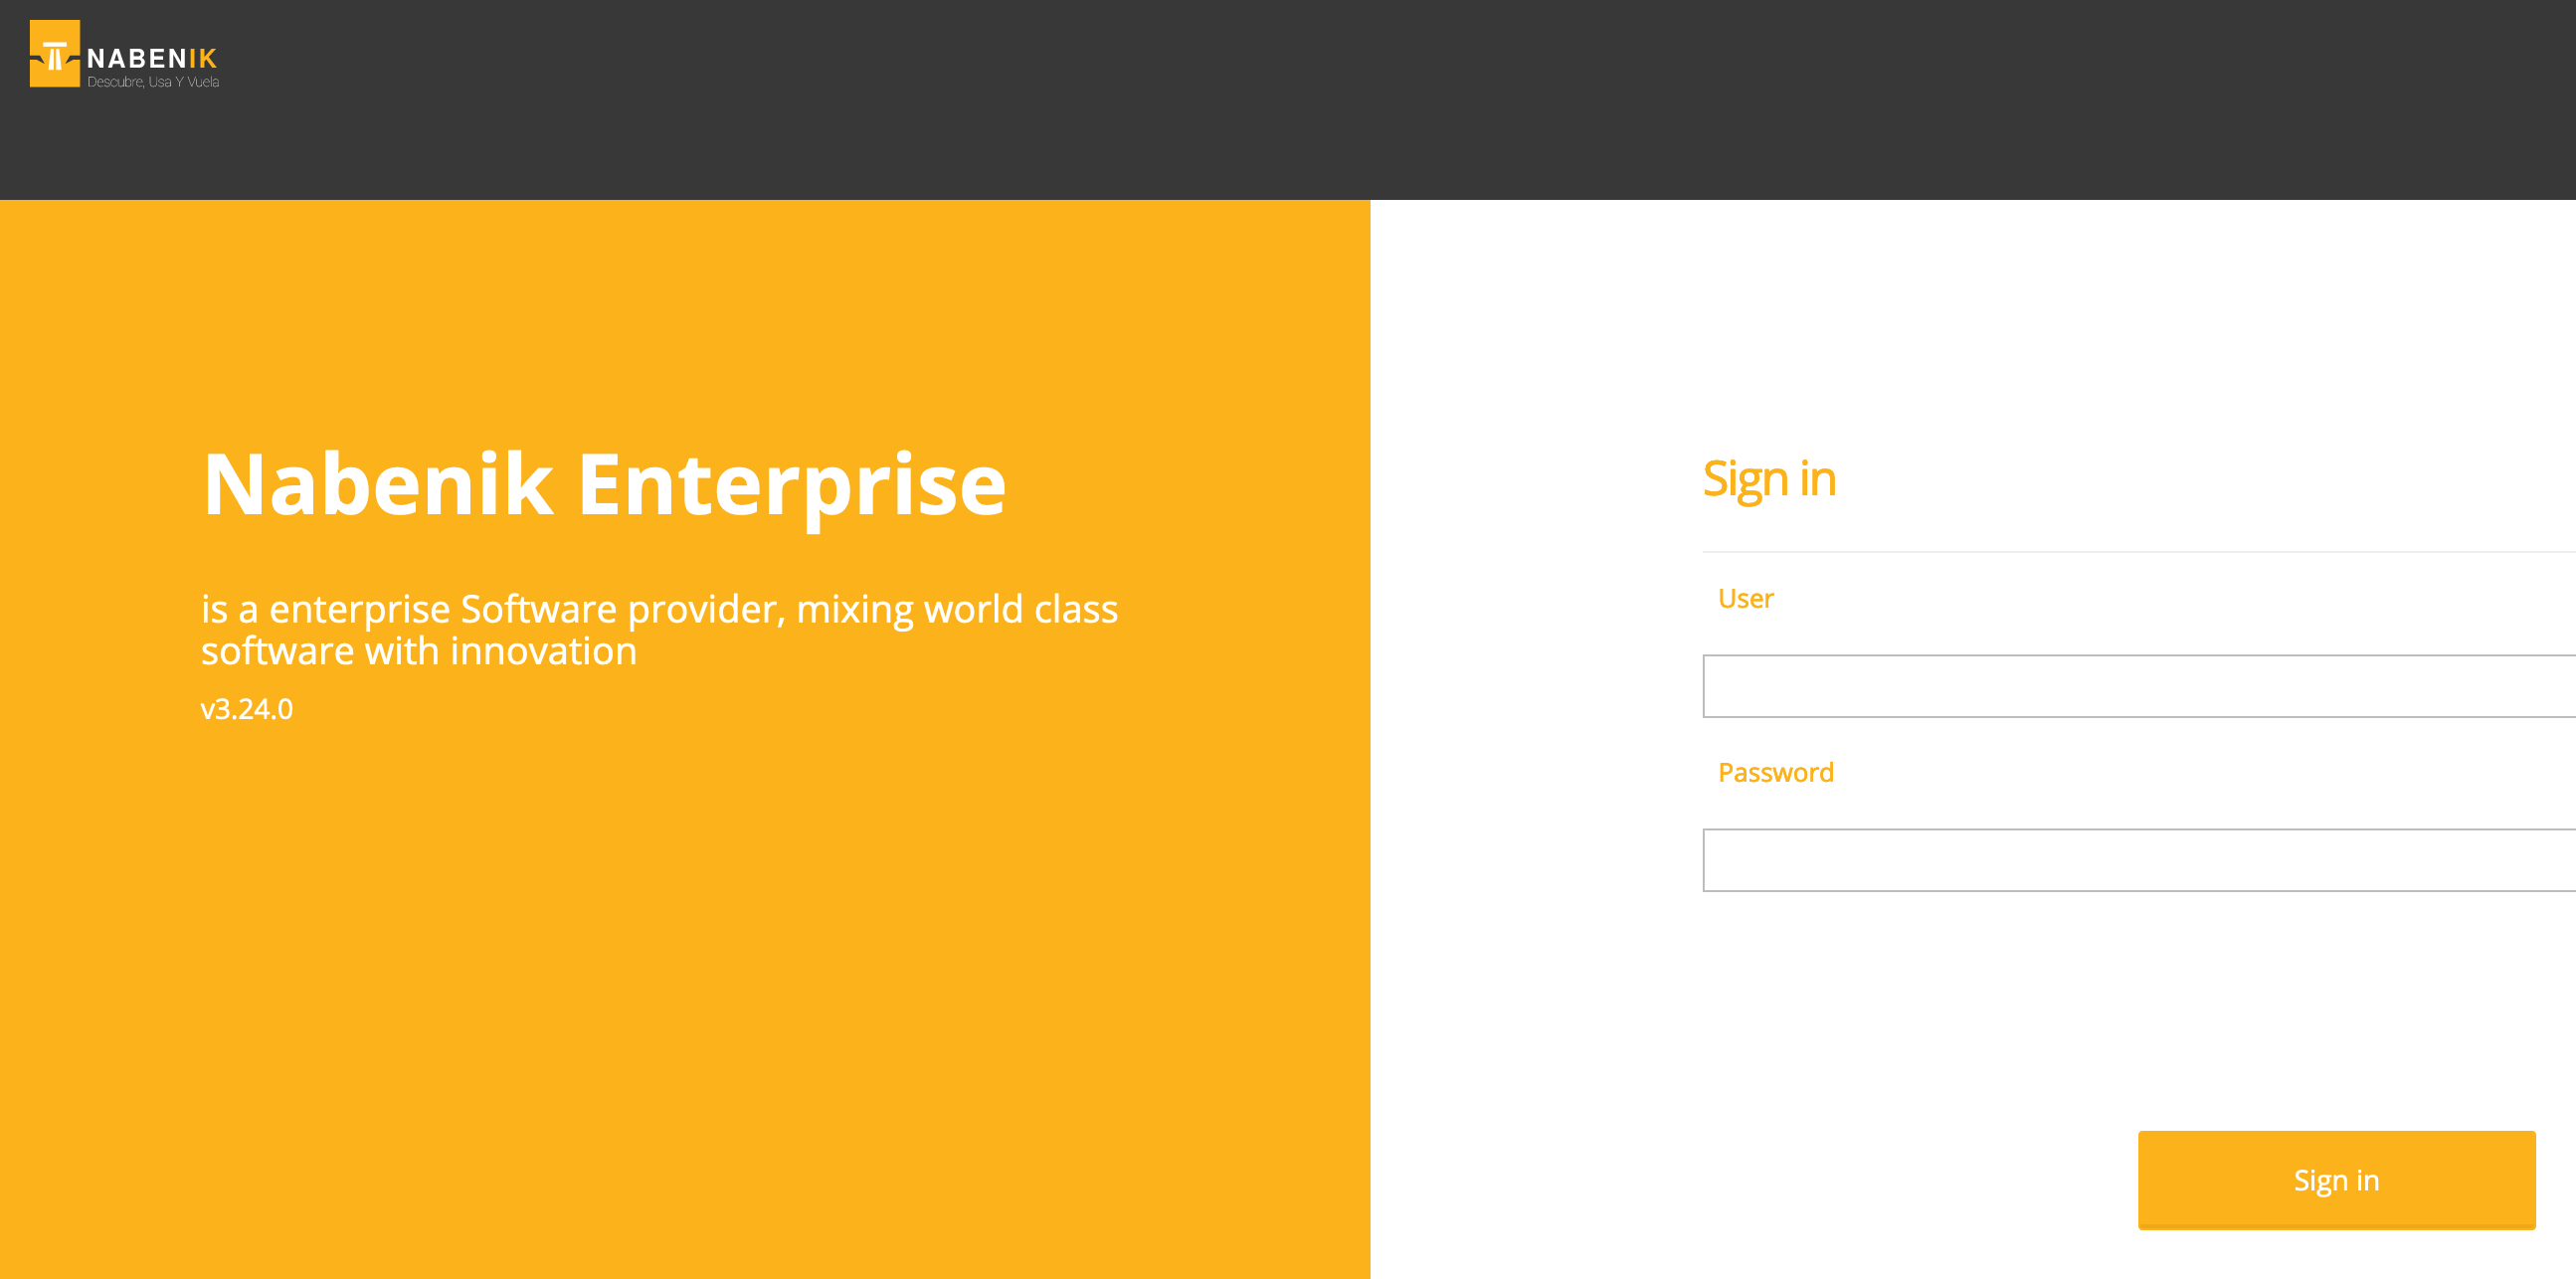
\includegraphics[width=\linewidth]{Images/erp}
    \end{figure}
\end{frame}


\begin{frame}[fragile]{Un - sistemita - contable y empresarial}
\begin{columns}[T] % contents are top vertically aligned

    \begin{column}[T]{5cm} % alternative top-align that's better for graphics
       \begin{itemize}
               \item 10 modulos (War, EJB, EAR)
               \item 671 clases
               \item 39480 lineas de código + dependencias
       \end{itemize}
    \end{column}
    \begin{column}[T]{6cm} % each column can also be its own environment
        \begin{itemize}
        \item 2014
           \item Original: Wildfly 8, Java EE 7, Java 7
           \item Actual: Wildfly 17, Jakarta EE 8, MicroProfile 3.0
           \item Cliente web (AngularJS)
       \end{itemize}
    \end{column}
\end{columns}
\end{frame}

\begin{frame}[fragile]{Un - sistemita - contable y empresarial}

    \begin{figure}
        \centering
        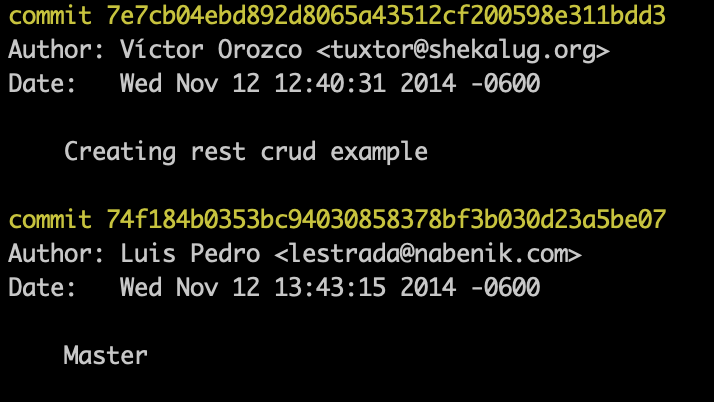
\includegraphics[width=0.7\linewidth]{Images/erpcommit1}
    \end{figure}
\end{frame}

\begin{frame}[fragile]{Un - sistemita - contable y empresarial}

    \begin{figure}
        \centering
        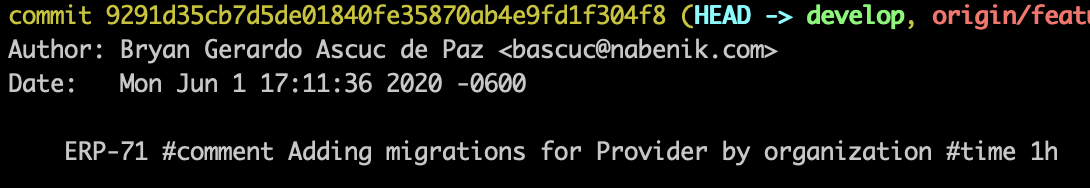
\includegraphics[width=\linewidth]{Images/erpcommit2}
    \end{figure}
\end{frame}


\begin{frame}[fragile]{Retos del mundo real}\scriptsize

Mi "mundo real"
    \begin{itemize}
        \item Venta/Geocerca (5 WAR) Payara Application Server
        \item ERP - 10 modulos (1 EAR, 9 EJB, 1 WAR), JBoss/Wildfly
        \item POS - JavaFX y Windows
    \end{itemize}
El rompe cabezas
\begin{itemize}
    \item Módulos en Java 9
    \item sun.misc.unsafe
    \item Corba y Java EE
    \item JavaFX
    \item IDE
    \item Licenciamiento
\end{itemize}
\end{frame}

{
    \usebackgroundtemplate{
\includegraphics[width=\paperwidth]{Images/separador}}
    \setbeamercolor{normal text}{fg=white}
    \setbeamercolor{frametitle}{fg=red}
    \usebeamercolor[fg]{normal text}
    \section{De Java 8 a Java 11}
}

\begin{frame}[fragile]{Algoritmo de actualización}
    Estrategia @tuxtor
    \begin{enumerate}
        \item Verificar y probar la compatibilidad del runtime/servidor/framework
        \item Múltiples JVM en desarrollo con cambio fácil
        \item Actualizar el compilador de Maven
        \item Actualizar las bibliotecas
        \item Incluir los módulos EE en los war/jar
        \item Actualizar el IDE
        \item Preparar el proyecto para módulos en el caso de JavaFX
        \item Determinar previamente el Java que necesito
        \item Ejecutar distintas versiones de Java en producción
    \end{enumerate}
\end{frame}

\begin{frame}[fragile]{Compatibilidad runtime}
    Compatibilidad con Java 11
    \begin{itemize}
        \item Tomcat
        \item Spring
        \item Micronaut
        \item Vert.x
        \item Jakarta EE (JBoss/Wildfly, OpenLiberty, Payara, WebLogic)
    \end{itemize}
\end{frame}

\begin{frame}[fragile]{Varias JVMs}
\begin{columns}[T] % contents are top vertically aligned

    \begin{column}[T]{5cm} % alternative top-align that's better for graphics
        \begin{figure}
            \centering
            
\includegraphics[width=\linewidth]{Images/jenv}
        \end{figure}
    \end{column}
    \begin{column}[T]{6cm} % each column can also be its own environment
        \begin{figure}
            \centering
            
\includegraphics[width=\linewidth]{Images/sdkman}
        \end{figure}
    \end{column}
\end{columns}
\end{frame}

\begin{frame}[fragile]{Bibliotecas}


    \begin{columns}[T] % contents are top vertically aligned

        \begin{column}[T]{5cm} % alternative top-align that's better for graphics
           Generación dinámica de Bytecode
               \begin{itemize}
                   \item ByteBuddy
                   \item ASM
                   \item glib
                   \item Spring
                   \item Java EE
                   \item Hibernate
                   \item Mockito
               \end{itemize}
        \end{column}
        \begin{column}[T]{7cm} % each column can also be its own environment
            \begin{figure}
                \centering
                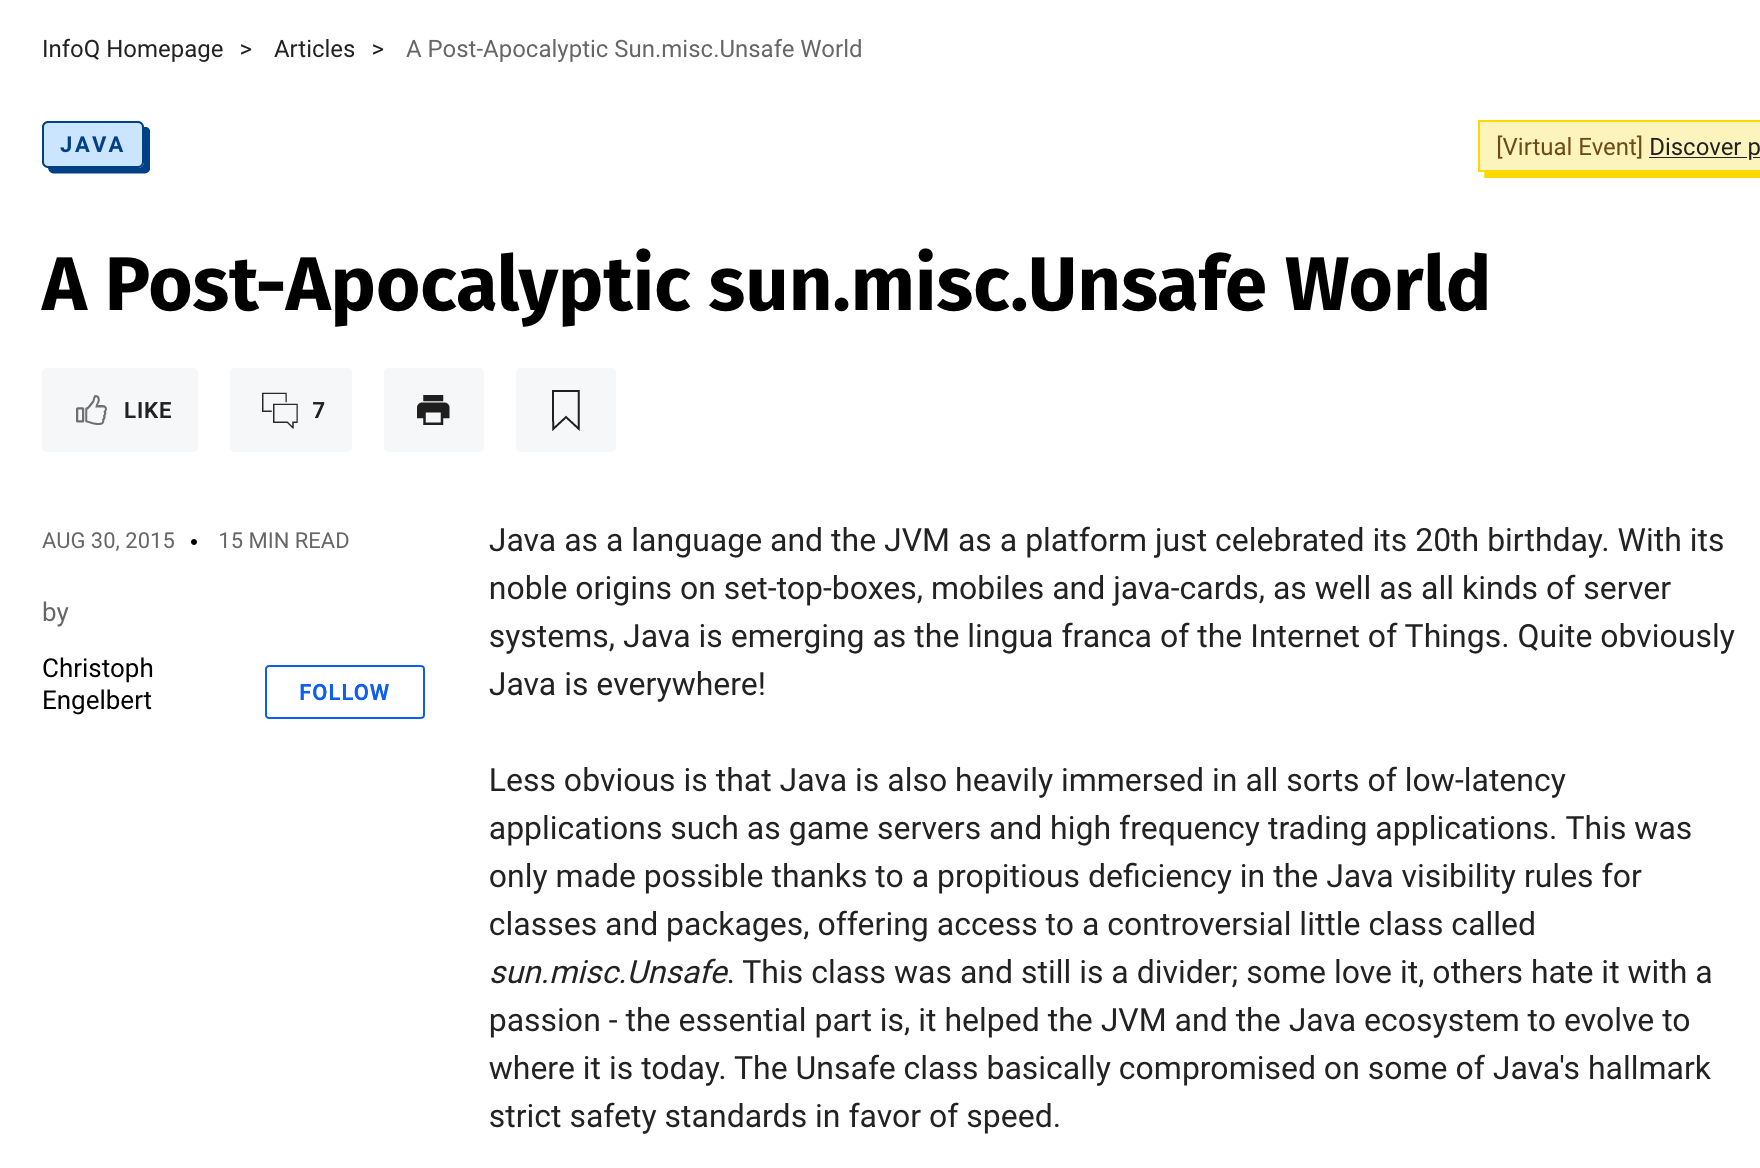
\includegraphics[width=\linewidth]{Images/sunmiscunsafe}
            \end{figure}
        \end{column}
    \end{columns}
\end{frame}

\begin{frame}[fragile]{Maven}
    \begin{itemize}
        \item Maven 3.5.0
        \item Compiler 3.8.0
        \item surefire 2.22.0
        \item failsafe 2.22.0
        \item release version 11.0
    \end{itemize}

\end{frame}


\begin{frame}[fragile]{Jakarta EE}

    \begin{figure}
        \centering
        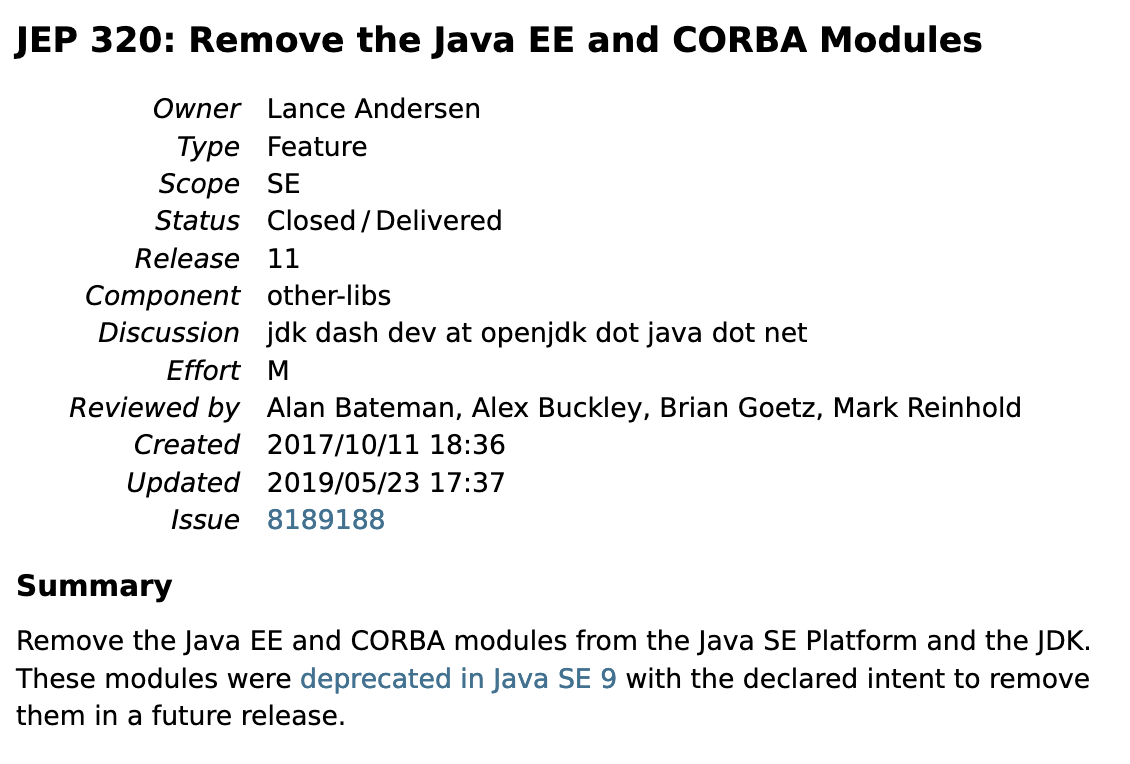
\includegraphics[width=0.7\linewidth]{Images/jep320}
    \end{figure}
\end{frame}


\begin{frame}[fragile]{Jakarta EE}

    \begin{figure}
        \centering
        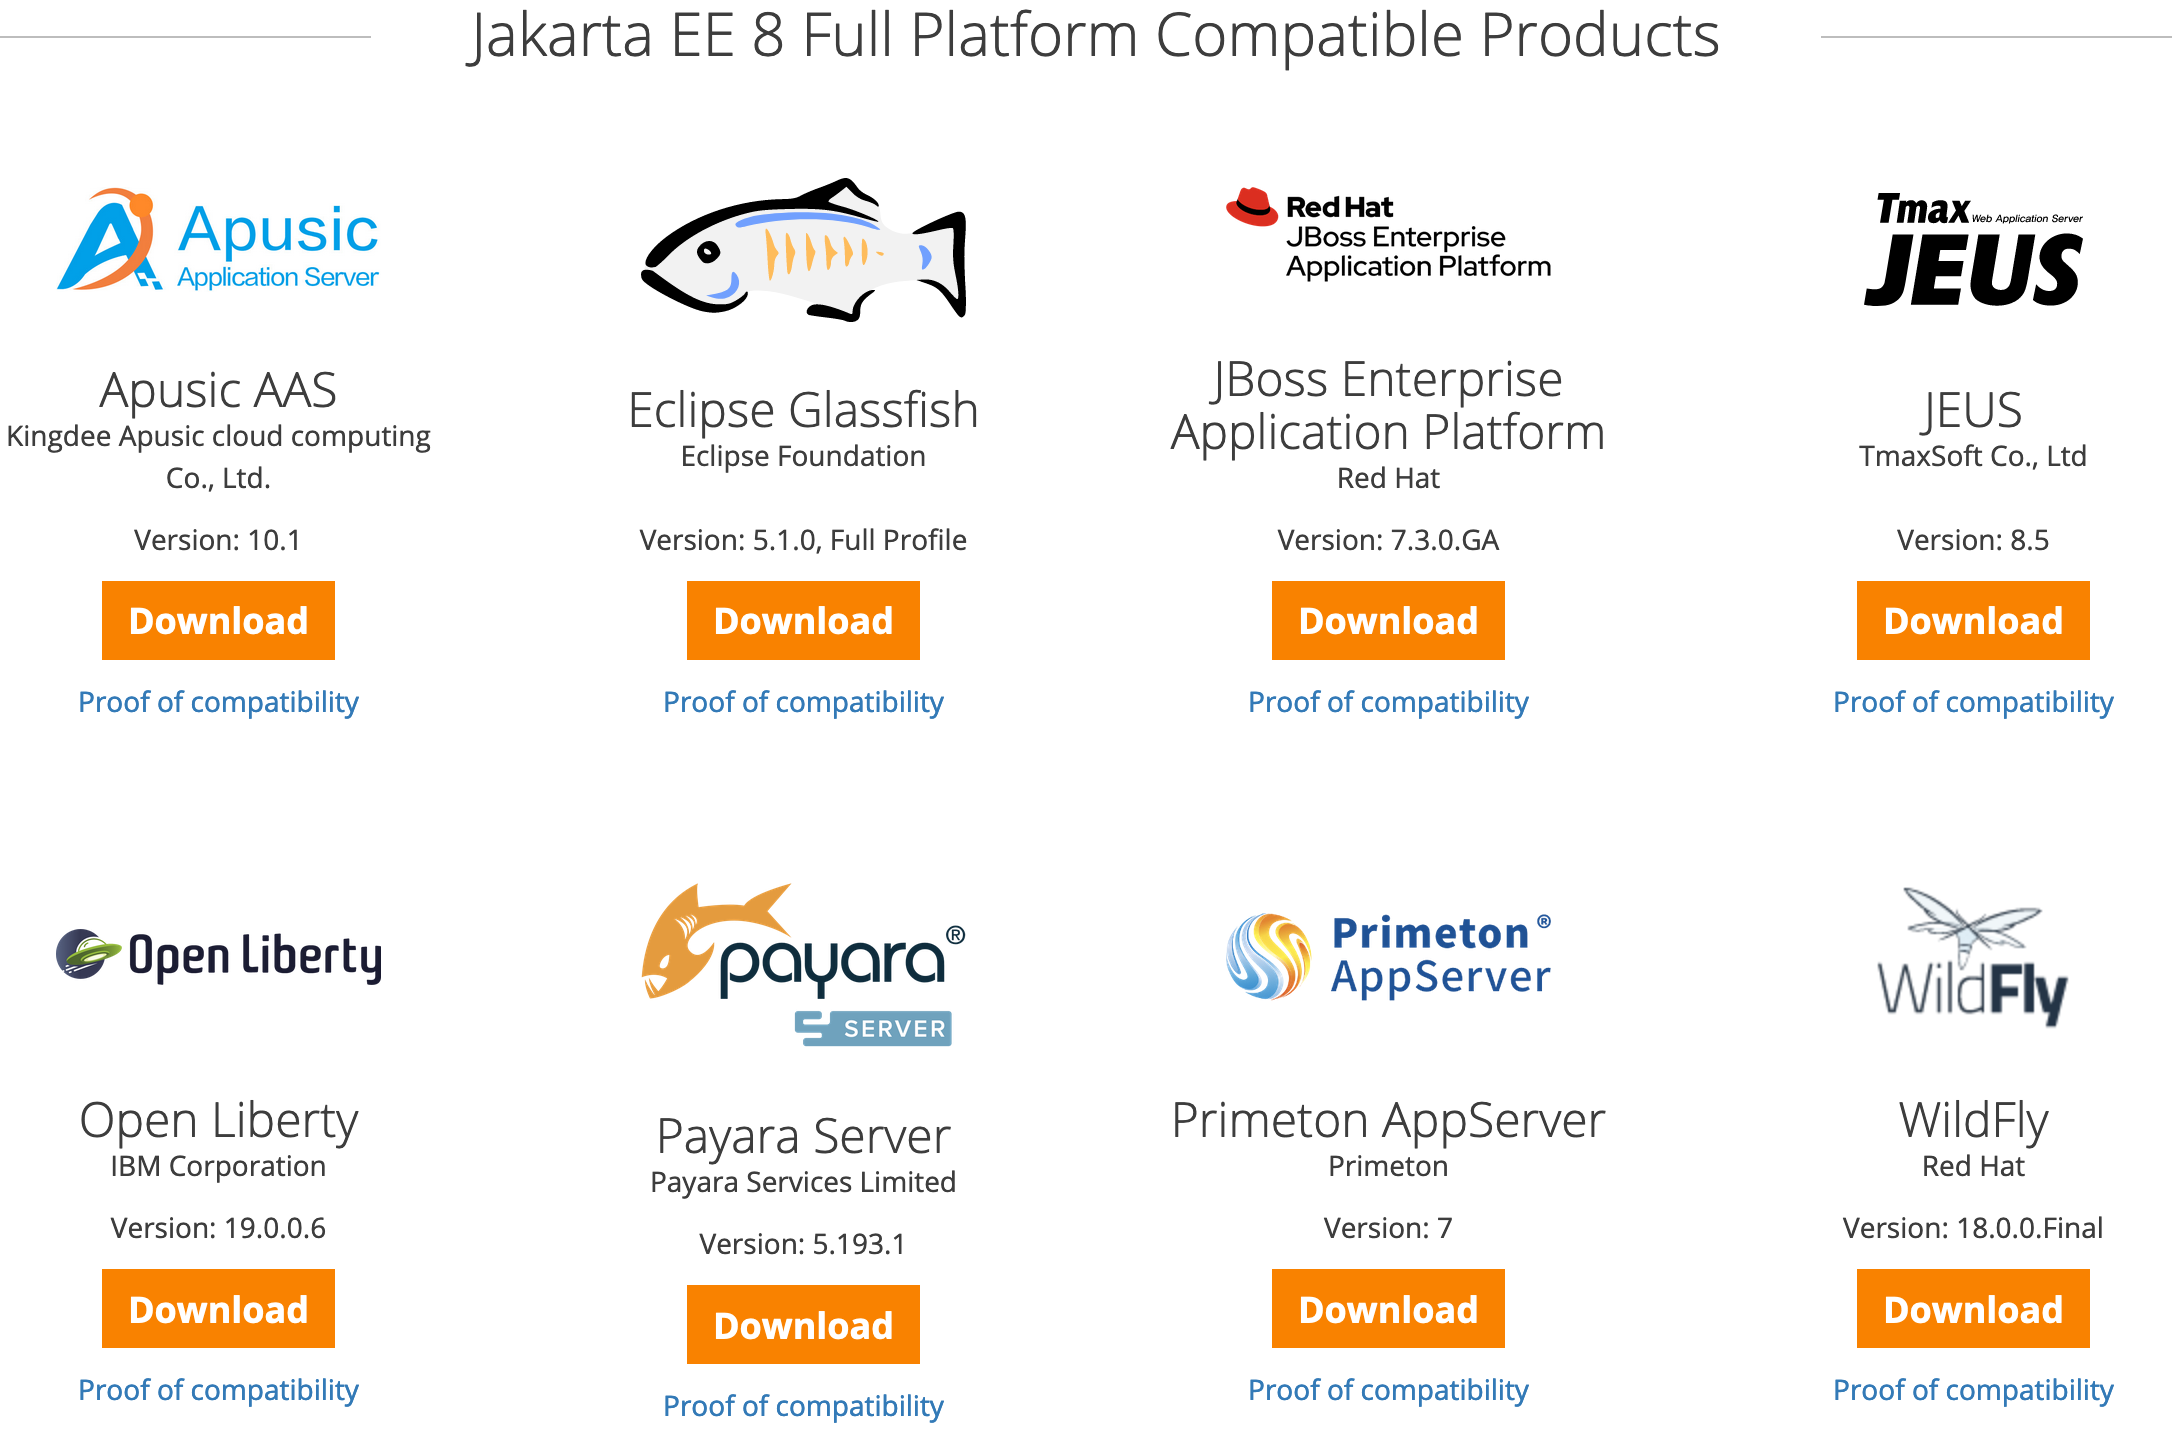
\includegraphics[width=\linewidth]{Images/jakarta}
    \end{figure}
\end{frame}


\begin{frame}[fragile]{Maven - Jakarta EE}
JAF (javax.activation)

\begin{lstlisting}[language=xml]
<dependency>
    <groupId>jakarta.activation</groupId>
    <artifactId>jakarta.activation-api</artifactId>
    <version>1.2.2</version>
</dependency>
\end{lstlisting}



CORBA = RIP
\end{frame}

\begin{frame}[fragile]{Maven - Jakarta EE}
JAXB (java.xml.bind)

\begin{lstlisting}[language=xml]
<!-- API -->
<dependency>
    <groupId>jakarta.xml.bind</groupId>
    <artifactId>jakarta.xml.bind-api</artifactId>
    <version>2.3.2</version>
</dependency>

<!-- Runtime -->
<dependency>
    <groupId>org.glassfish.jaxb</groupId>
    <artifactId>jaxb-runtime</artifactId>
    <version>2.3.2</version>
</dependency>
\end{lstlisting}
\end{frame}

\begin{frame}[fragile]{Maven - Jakarta EE}
    JAX-WS (java.xml.ws)

\begin{lstlisting}[language=xml]
<!-- API -->
<dependency>
    <groupId>jakarta.xml.ws</groupId>
    <artifactId>jakarta.xml.ws-api</artifactId>
    <version>2.3.2</version>
</dependency>

<!-- Runtime -->
<dependency>
    <groupId>com.sun.xml.ws</groupId>
    <artifactId>jaxws-rt</artifactId>
    <version>2.3.2</version>
</dependency>
\end{lstlisting}
\end{frame}

\begin{frame}[fragile]{Maven - Jakarta EE}
Common Annotations (java.xml.ws.annotation)

\begin{lstlisting}[language=xml]
<dependency>
    <groupId>jakarta.annotation</groupId>
    <artifactId>jakarta.annotation-api</artifactId>
    <version>1.3.5</version>
</dependency>
\end{lstlisting}
\end{frame}

\begin{frame}[fragile]{IDEs}

    IDEs compatibles con Java 11
    \begin{itemize}
        \item Eclipse
        \item NetBeans
        \item IntelliJ IDEA
        \item Visual Studio Code
    \end{itemize}

    Algunos plug-ins problemáticos
    \begin{enumerate}
        \item Glassfish
        \item WebLogic
        \item Icefaces
    \end{enumerate}
\end{frame}

\begin{frame}[fragile]{JavaFX}

    JavaFX es un módulo independiente del JDK a partir de Java 11, compatible con JPMS, casi todos usan la compilación de Gluon
    \begin{figure}
        \centering
        
\includegraphics[width=\linewidth]{Images/gluon}
    \end{figure}
\end{frame}

\begin{frame}[fragile]{¿Cual Java necesito?}
    Obligatorios por contrato
    \begin{itemize}
        \item Software comercial de Oracle (HotSpot)
        \item Software comercial de SAP (SAP VM)
        \item Software comercial de Red Hat (OpenJDK + RHEL)
        \item Software comercial de IBM (J9)
    \end{itemize}
    Algunos otros "Javas"
\begin{itemize}
    \item AdoptOpenJDK (soporte de IBM en J9)
    \item Correto
    \item Azul Zulu
    \item Java en Linux
\end{itemize}
\end{frame}

\begin{frame}[fragile]{Varias JVM en producción}
    Linux
    \begin{itemize}
        \item Docker
        \item RHEL
        \item Oracle Linux
        \item Debian
        \item Gentoo
    \end{itemize}
    Windows
    \begin{itemize}
        \item Docker / Containerd
        \item Variables de entorno en proyecto/runtime
        \item Lo importante es la salud
    \end{itemize}
\end{frame}

{
    \usebackgroundtemplate{
\includegraphics[width=\paperwidth]{Images/separador}}
    \setbeamercolor{normal text}{fg=white}
    \setbeamercolor{frametitle}{fg=red}
    \usebeamercolor[fg]{normal text}
    \section{De mi data center a la nube - moderna -}
}


\begin{frame}[fragile]{Desde mi data center}
    \begin{figure}
        \centering
        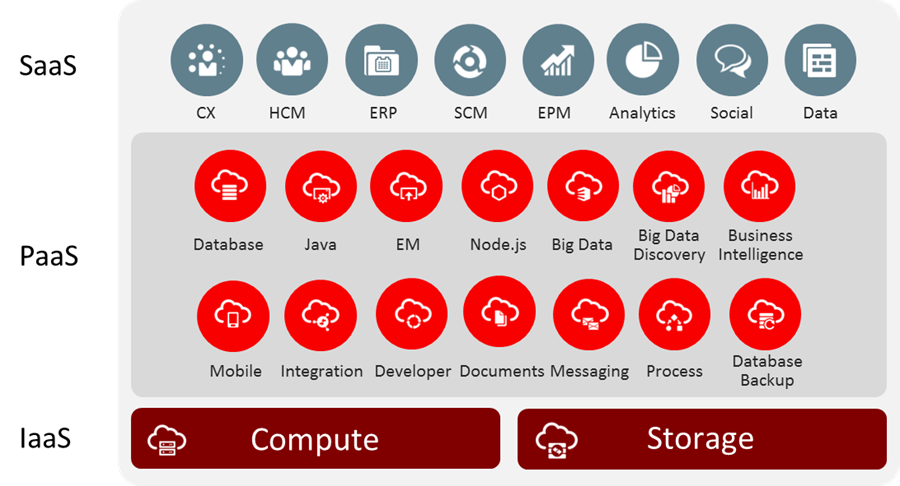
\includegraphics[width=\linewidth]{Images/cloud}
    \end{figure}
\end{frame}



\begin{frame}[fragile]{Desde mi data center}


    \begin{columns}[T] % contents are top vertically aligned

        \begin{column}[T]{5cm} % alternative top-align that's better for graphics
            PaaS
               \begin{itemize}
                   \item Clasico: Desplegar War en servidores autonomos
                   \item Primer abordaje: Desplegar contenedores de forma manual

                   \item Abordaje maduro: Desplegar contenedores y orquestar con Rancher/Docker Swarm/Kubernetes/Mesos
               \end{itemize}
        \end{column}
        \begin{column}[T]{7cm} % each column can also be its own environment
            \begin{figure}
                \centering
                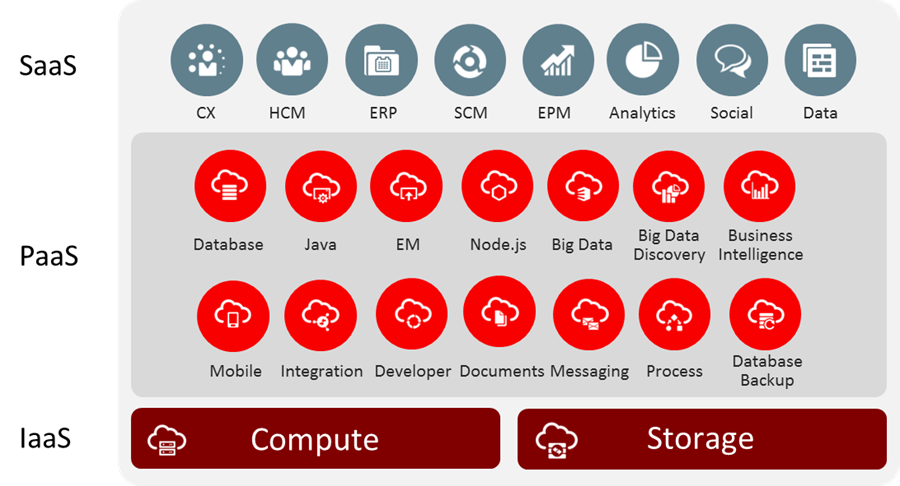
\includegraphics[width=\linewidth]{Images/cloud}
            \end{figure}
        \end{column}
    \end{columns}
\end{frame}

\begin{frame}[fragile]{Desde mi data center}
    \begin{figure}
        \centering
        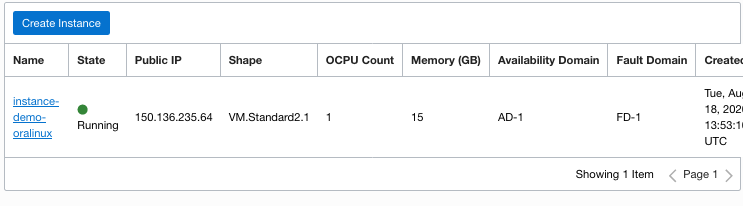
\includegraphics[width=\linewidth]{Images/oracloud}
    \end{figure}
\end{frame}

{
    \usebackgroundtemplate{
\includegraphics[width=\paperwidth]{Images/separador}}
    \setbeamercolor{normal text}{fg=white}
    \setbeamercolor{frametitle}{fg=red}
    \usebeamercolor[fg]{normal text}
    \section{Desdse Java 14 hasta el infinito}
}


\begin{frame}[fragile]{¿Que recibo con cada versión nueva de Java?}
	\begin{itemize}
		\item Java - \textbf{Lenguaje}
		\item Java - Bibliotecas e APIs
		\item Java - Maquina Virtual de Java
	\end{itemize}
\end{frame}



\begin{frame}[fragile]{Java - Las mejoras que resaltan}
	\begin{columns}[T] % contents are top vertically aligned

		\begin{column}[T]{5cm} % alternative top-align that's better for graphics
			\begin{itemize}
				\item Java 9
				\begin{itemize}
					\item Modulos
					\item JShell
					\item HTTP/2
                    \item Factory methods
				\end{itemize}
				\item Java 10
				\begin{itemize}
					\item Type Inference
					\item Class Data Sharing
					\item Time based release
				\end{itemize}
			\end{itemize}
		\end{column}
		\begin{column}[T]{5cm} % each column can also be its own environment
			\begin{itemize}
                \item Java 11
                \begin{itemize}
                    \item String methods
                    \item File methods
                    \item Direct .java execution
                \end{itemize}
				\item Java 12
				\begin{itemize}
					\item Switch expressions
				\end{itemize}
				\item Java 13
				\begin{itemize}
					\item Text blocks
				\end{itemize}
				\item Java 14
				\begin{itemize}
					\item Pattern matching
					\item Records
					\item Helpfull NPE
				\end{itemize}
			\end{itemize}
		\end{column}
	\end{columns}
\end{frame}

\begin{frame}[fragile]{JEP 110: HTTP/2 Client }
\begin{lstlisting}
HttpRequest request = HttpRequest.newBuilder()
    .uri(new URI("https://swapi.co/api/starships/9"))
    .GET()
    .build();

HttpResponse<String> response = HttpClient.newHttpClient()
    .send(request, BodyHandlers.ofString());

System.out.println(response.body());
\end{lstlisting}
\end{frame}


\begin{frame}[fragile]{JEP 286: Local-Variable Type Inference}
\begin{lstlisting}
public static void main(String args[]){
    var localValue = 99;
    System.out.println(++localValue);
    //localValue = "Foo"
}
\end{lstlisting}
\end{frame}

\begin{frame}[fragile]{JEP 330: Launch Single-File Source-Code Programs}
    \begin{figure}
        \centering
        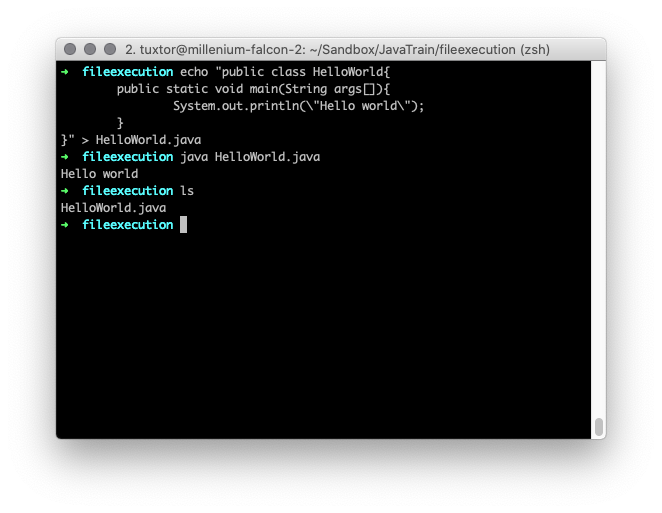
\includegraphics[width=0.9\linewidth]{Images/jep222singlefile}
    \end{figure}

\end{frame}

\begin{frame}[fragile]{325: Switch Expressions (Preview)}
Ahora
\begin{lstlisting}
String langType = switch (args[0]) {
    case "Java", "Scala", "Kotlin" -> "Static typed";
    case "Groovy", "JavaScript" -> "Dynamic typed";
    default -> {
        System.out.println("This meant to be a processing block");
        yield "Probably LISP :)";
    }
};
System.out.println(langType);
\end{lstlisting}
\end{frame}

\begin{frame}[fragile]{355: Text Blocks (Preview)}
Antes
\begin{lstlisting}
String html = "<html>\n" +
"    <body>\n" +
"        <p>Hello, world</p>\n" +
"    </body>\n" +
"</html>\n";
\end{lstlisting}

Ahora
\begin{lstlisting}
String html = """
<html>
    <body>
        <p>Hello, world</p>
    </body>
</html>
""";
\end{lstlisting}
\end{frame}

\begin{frame}[fragile]{JEP 359: Records (Preview)}
Data carrier
\begin{lstlisting}
record Person(String name, String email, int age) {}
\end{lstlisting}

Uso
\begin{lstlisting}
Person foo = new Person("Marco", "example@mail.com",99);
System.out.println(foo);
//foo.name = "Polo";
\end{lstlisting}
\end{frame}



\begin{frame}{Víctor Orozco}
\begin{columns}[T] % contents are top vertically aligned

	\begin{column}[T]{4cm} % alternative top-align that's better for graphics
		\begin{figure}
			\centering
			
\includegraphics[width=\linewidth]{Images/logos}
		\end{figure}
	\end{column}
	\begin{column}[T]{6cm} % each column can also be its own environment
		\begin{itemize}
			\item vorozco@nabenik.com
			\item \href{https://twitter.com/tuxtor}{@tuxtor}
			\item \href{http://vorozco.com}{http://vorozco.com}
			\item \href{http://tuxtor.shekalug.org}{http://tuxtor.shekalug.org}
		\end{itemize}
		\begin{center}
			
\includegraphics[width=0.1\linewidth]{Images/cclogo}
			\\
			This work is licensed under Creative Commons Attribution-NonCommercial-ShareAlike 3.0 Guatemala (CC BY-NC-SA 3.0 GT).
		\end{center}
	\end{column}
\end{columns}
\end{frame}

\end{document}

